\chapter{The 3-2-1 Speaking Trick That Forces You To Stop Rambling!}

We begin with a practical puzzle. How do we train the mind to think faster when we are put on the spot? Zhang does not answer by giving us motivational advice or by asking for more confidence in the abstract. He begins with the failure mode, isolates the point at which speech breaks down, and then introduces a very small framework that can be reached for under pressure. The lecture therefore unfolds as a controlled argument: diagnose the disorder, replace disorder with structure, and then test that structure on live examples.

\section{The Opening Problem}

The lecture opens with a question: what happens when someone asks us something and we are not prepared? The answer is not merely that we feel nervous. It is that thought branches too quickly. The mind opens too many possible directions, and speech begins before any one line has been selected and stabilized. In the language of these notes, the opening causal chain is
\begin{equation}
\text{unprepared question}
\;\Rightarrow\;
\text{panic search}
\;\Rightarrow\;
\text{rambling}.
\end{equation}
That is the first real structure in the lecture. Rambling is not the primitive problem; it is the visible consequence of a deeper disorder in the search process.

Zhang immediately gives this diagnosis weight by making it personal. He says he used to do this. The result, as he describes it, is not just verbal messiness but a collapse in confidence: we feel incompetent, we look less confident than we are, and the whole exchange becomes frustrating or embarrassing. This matters because the lecture is not really about clever phrasing. It is about what happens when speech outruns structure.

\subsection{Question \& Answer}

\paragraph{Question.} Why do we ramble when we are put on the spot?

\paragraph{Answer.} Because speech begins before thought has found an organizing line. Zhang's image is that the brain opens ``a dozen browser tabs.'' That is exactly the right picture: too many candidate directions appear at once, and instead of choosing one and building from it, we start talking in the middle of the search. Rambling is therefore a structural failure, not simply a temperamental one.

\section{From Panic to Fallback}

Only after diagnosing the disorder does Zhang pivot to the solution. He contrasts prepared content with off-the-cuff speaking: when content is prepared, confidence rises; when one is forced to improvise, confidence falls. He then asks the decisive question: if we are not prepared, what do we fall back on?

His answer is blunt. Generally, we fall back on rambling. This is the moment in the lecture where the main object becomes necessary. A framework is not introduced as decoration; it is introduced as a fallback mechanism:
\begin{equation}
\text{no framework}
\;\Rightarrow\;
\text{fallback to rambling},
\qquad
\text{framework}
\;\Rightarrow\;
\text{fallback to structure}.
\end{equation}
That equation is the hinge of the chapter. Once we see it, the rest of the lecture follows naturally. The problem is not that we lack words. The problem is that under pressure we lack a small structure that can be reached for immediately.

Zhang briefly checks the room: how many people already use frameworks when they communicate? The point of that check is not statistical precision; it is pedagogical contrast. Most people do not consciously use them. So the lecture now introduces a particularly simple one.

\section{The \texorpdfstring{$3,2,1$}{3,2,1} Framework}

Zhang names the framework before he explains it. That is why the opening board matters. The lecture first presents \((3,2,1)\) as an object and only then unfolds its meaning.

\begin{figure}[h]
\centering

\includegraphics[width=0.72\textwidth]{lecture_13_figure_01.png}
\caption{Opening board: \((3,2,1)\) is introduced explicitly as a framework.}
\end{figure}

The visible board label is minimal and direct:
\begin{equation}
\left(3,2,1\right),
\qquad
\left[\text{Framework}\right].
\end{equation}
This is not yet a derivation. It is an announcement: we are being given a named object that can later be used operationally.

\begin{figure}[h]
\centering
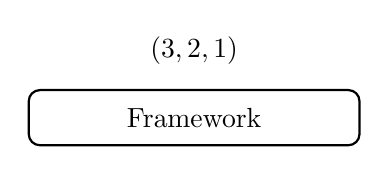
\begin{tikzpicture}[x=1cm,y=1cm]
\node at (0,1.45) {$\left(3,2,1\right)$};
\draw[thick,rounded corners] (-2.1,0.25) rectangle (2.1,0.95);
\node at (0,0.60) {Framework};
\end{tikzpicture}
\caption{Minimal reconstruction of the opening board label.}
\end{figure}

Zhang then repeats the definition in speech, and the repetition matters. ``Three, two, one means what? It means three steps, two types, and the one thing.'' Then he says it again: ``Three steps, two types, one thing.'' We should preserve that fixed order:
\begin{equation}
3\ \text{steps},\ 2\ \text{types},\ 1\ \text{thing}.
\end{equation}

\begin{definition}
For a topic \(T\), we may represent the lecture's scaffold editorially by
\begin{equation}
F_{321}(T)
=
\bigl(
\text{3 steps for }T,\;
\text{2 types of }T,\;
\text{1 thing about }T
\bigr).
\end{equation}
This notation is introduced for clarity in the notes. It is not written by Zhang on the board.
\end{definition}

At once, however, Zhang makes a practical refinement that is crucial. Although the framework is named in the order \(3,2,1\), one need not enter it from the first slot. One may begin where the mind can get traction most quickly:
\begin{equation}
\text{entry}(F_{321}(T))
\in
\left\{
\text{1 thing about }T,\;
\text{2 types/ways of }T,\;
\text{3 steps for }T
\right\}.
\end{equation}
This is why the framework is usable under pressure. It is not a rigid script. It is a small menu of admissible decompositions.

The lecture also motivates the framework by use. Zhang says he still uses it, that he is using it in this very Q\&A, that he uses it for social media content, and that he uses it whenever he has very little time to prepare. These remarks do not add new notation, but they explain why the framework deserves attention: it is not a classroom curiosity but a live instrument.

\subsection{Question \& Answer}

\paragraph{Question.} What exactly does \(3,2,1\) mean?

\paragraph{Answer.} In the strict lecture order it means three steps, two types, one thing. But the deeper point is that it gives us three small answer shapes. Instead of searching the whole topic at once, we choose one admissible shape and begin there. The framework is therefore not a slogan to memorize but a compact family of decompositions.

\section{A Worked Example: Avocado}

Having defined the framework, Zhang immediately tests it. He asks the audience for a random topic and receives ``avocado.'' This is an important beat in the lecture. The framework is not left hanging in abstraction. It is stress-tested on an arbitrary topic.

The workshop boards give the clearest visual summary of the scaffold.

\begin{figure}[h]
\centering

\includegraphics[width=0.82\textwidth]{lecture_13_figure_03.png}
\caption{Workshop boards: the left board shows the \(3,2,1\) scaffold; the right board shows a second staged framework.}
\end{figure}

The left board gives the visible structure already stated in speech:
\begin{equation}
3\ \text{steps},\ 2\ \text{types},\ 1\ \text{thing}.
\end{equation}
The right board shows a separate framework headed by \(\#\text{Framework}\), with visible stages \(S_1,S_2,S_3,S_4\) and a downward directional cue. The long handwritten stage labels are not secure enough to transcribe, but the staged motion itself is clear enough to preserve cautiously:
\begin{equation}
S_1 \to S_2 \to S_3 \to S_4.
\end{equation}
This right-hand board is secondary to the lecture's main line, but it matters visually because it reminds us that Zhang is thinking in terms of frameworks as a class, not just in terms of one isolated trick.

\begin{figure}[h]
\centering
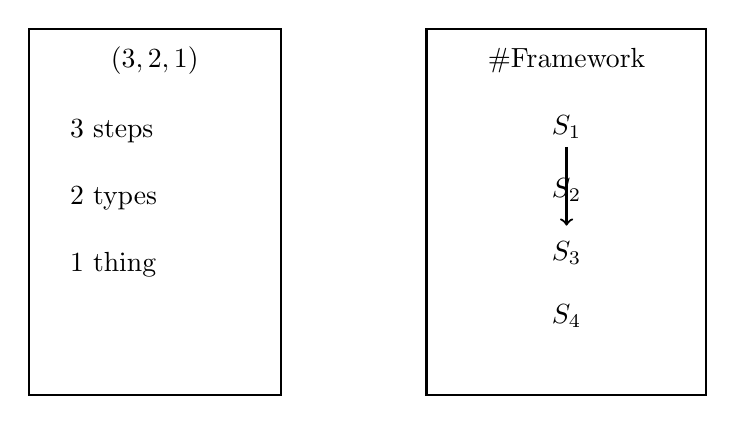
\begin{tikzpicture}[x=1cm,y=1cm]
\draw[thick] (-4.9,-0.2) rectangle (-1.7,4.45);
\node at (-3.3,4.05) {$\left(3,2,1\right)$};
\node[anchor=west] at (-4.5,3.15) {$3$ steps};
\node[anchor=west] at (-4.5,2.30) {$2$ types};
\node[anchor=west] at (-4.5,1.45) {$1$ thing};

\draw[thick] (0.15,-0.2) rectangle (3.7,4.45);
\node at (1.93,4.05) {\#Framework};
\node at (1.93,3.20) {$S_1$};
\node at (1.93,2.40) {$S_2$};
\node at (1.93,1.60) {$S_3$};
\node at (1.93,0.80) {$S_4$};
\draw[->,thick] (1.93,2.95) -- (1.93,1.95);
\end{tikzpicture}
\caption{Clean reconstruction of the visible board structure. The detailed labels on the right board are omitted because they are not reliably legible.}
\end{figure}

Now let us follow the avocado example in the order it is actually performed. Zhang does not start with ``three steps.'' He starts with the easiest slot, the one thing. In that sense the lecture performs the flexibility encoded above. We can record the example compactly as
\begin{equation}
F_{321}(\text{avocado})
=
\bigl(
\text{3 preparation steps},
\text{2 ways to have it},
\text{1 thing about it}
\bigr),
\end{equation}
but the live execution enters through the last component first.

The worked reduction looks like this:
\begin{align}
\text{1 thing} &:\ \text{avocado is, for him, excellent on a keto diet},\\
\text{2 ways} &:\ \text{smash it on toast, or eat it like a fruit},\\
\text{3 steps} &:\ \text{cut it, mash it, add seasoning}.
\end{align}
This is the lecture's first full demonstration of the framework in motion.

The contrast with disorder is equally important. Zhang does not merely show the successful path; he dramatizes the uncontrolled alternative. Without a framework the mind spins through one possible line after another: color, ripeness, storage, recipes, whether it can still be eaten, what one should mix into it. In shorthand,
\begin{equation}
\text{avocado}
\;\Rightarrow\;
\{\text{green},\text{ripe},\text{storage},\text{recipes},\ldots\}
\;\Rightarrow\;
\text{blankness or tongue-twisting}.
\end{equation}
The framework works because it narrows the search. We do not have to search the whole topic space. We only have to choose one of a few permissible forms.

\subsection{Question \& Answer}

\paragraph{Question.} How does the framework give the brain something to lean on?

\paragraph{Answer.} It reduces the number of live options. Instead of facing an undifferentiated topic and searching everywhere at once, we collapse the topic into one of three small shapes: one thing, two types, or three steps. The mind can then begin constructing rather than searching blindly.

There is also a subtle refinement in this example. Zhang locally relaxes ``two types'' into ``two ways.'' That is not a contradiction. It is part of the point. The second slot is broad enough to host a classification or a small contrast. The third slot, by contrast, gives an explicitly procedural decomposition. So the same framework can support both descriptive and sequential speech.

\section{Pressure, Pause, and the Wider Family of Frameworks}

At this point the lecture turns to its next tension. The viewer is meant to think: fine, that worked for the lecturer, but can I do it? Zhang anticipates this reaction directly. He answers, yes, because the viewer is going to do it. He then brings up a student, and before giving the topic he removes a possible source of pressure: the student need not do all three. She may pick whichever one is easiest.

That detail should not be lost. The framework is not a demand for maximal output. It is a permission structure:
\begin{equation}
\text{pick one admissible slot first}
\;\Rightarrow\;
\text{stabilize the answer}
\;\Rightarrow\;
\text{expand only if needed}.
\end{equation}
He also says, when the student admits she is not ready, that no one is ever ready. This too is a precise motivational move. The lecture does not promise that pressure disappears. It promises that pressure can be met with a structure.

Before the drill concludes, the lecture briefly pauses to remind us that \(3,2,1\) is only one communication framework among several. The visual evidence for this broader placement is the inserted board shot.

\begin{figure}[h]
\centering

\includegraphics[width=0.78\textwidth]{lecture_13_figure_04.png}
\caption{Inserted board shot: the \(3,2,1\) scaffold appears under a broader heading, indicating a larger family of frameworks.}
\end{figure}

What is reliable here is the board hierarchy, not the promotional banner at the bottom, which we set aside. The visible upper structure is
\begin{equation}
\text{Visibility},
\qquad
2)\ \left(3,2,1\right).
\end{equation}
Below it sits the now familiar scaffold, and colored connector lines run toward a right-hand annotation whose exact wording is uncertain. The safest reading is simply that \(3,2,1\) is being placed inside a wider inventory of communication tools.

\begin{figure}[h]
\centering
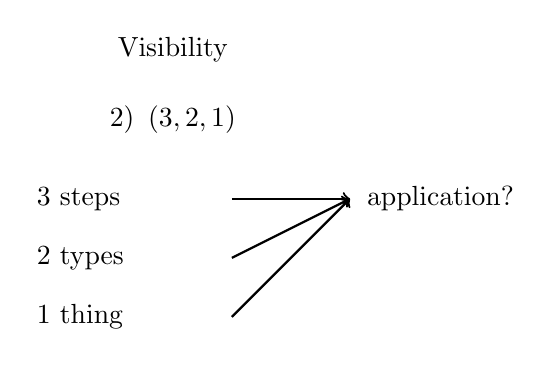
\begin{tikzpicture}[x=1cm,y=1cm]
\node at (0,3.85) {Visibility};
\node at (0,2.95) {$2)\ \left(3,2,1\right)$};

\node[anchor=west] at (-1.85,1.95) {$3$ steps};
\node[anchor=west] at (-1.85,1.20) {$2$ types};
\node[anchor=west] at (-1.85,0.45) {$1$ thing};

\draw[->,thick] (0.75,1.95) -- (2.25,1.95);
\draw[->,thick] (0.75,1.20) -- (2.25,1.95);
\draw[->,thick] (0.75,0.45) -- (2.25,1.95);
\node at (3.4,1.95) {application?};
\end{tikzpicture}
\caption{Conservative reconstruction of the visible board hierarchy. The right-hand application label is left generic because the handwriting is not fully secure.}
\end{figure}

\subsection{Question \& Answer}

\paragraph{Question.} Must we use all three parts of the framework every time?

\paragraph{Answer.} No. Zhang says explicitly that one may pick whichever one is easiest. This is not a minor convenience; it is the operative rule that makes the framework usable under pressure. The scaffold is a way to begin, not a burden to complete in full on every occasion.

\section{Travel: Transfer Under Time Pressure}

Only now does the lecture resolve the live tension it has created. The random topic is ``travel.'' Zhang counts down: three, two. The student answers before the count is even finished. That quickness is part of the proof. The framework has become available quickly enough to change the tempo of the exchange.

If we write the response in the lecture's structural order, we have
\begin{equation}
F_{321}(\text{travel})
=
\bigl(
\text{plan it, book it, go},
\text{regional or international},
\text{travel is magnificent}
\bigr).
\end{equation}
If we write it in the order in which the student actually performs it, we get the operational sequence
\begin{align}
\text{1 thing} &:\ \text{travel is magnificent; you can go anywhere you want},\\
\text{2 types} &:\ \text{regional travel and international travel},\\
\text{3 steps} &:\ \text{plan it, book it, go}.
\end{align}
This is the transfer test, and the transfer succeeds.

The lecture then turns back to interpretation. Without frameworks, Zhang says, the brain would again spin into disorder: what do you mean travel, I hate travel, I do not want to bother the kids, and so on. The framework prevents precisely that collapse. But Zhang's final point goes beyond verbal neatness. He notes the student's body language. She leaned into the microphone and moved toward the task. This is why the closing structure of the lecture should be written as
\begin{equation}
\text{framework}
\;\Rightarrow\;
\text{readiness}
\;\Rightarrow\;
\text{confident communication}.
\end{equation}
The framework changes more than the sentence. It changes the posture from which the sentence is spoken.

\subsection{Question \& Answer}

\paragraph{Question.} Why does a framework change not only what we say, but how ready we feel?

\paragraph{Answer.} Because once a stable answer shape is available, speech no longer feels like a leap into chaos. The framework reduces uncertainty before the first sentence is spoken. That cognitive reduction becomes visible as bodily readiness: the speaker steps forward, leans in, and communicates with less hesitation.

\section{Summary}

The lecture unfolds in a clean order. First, it diagnoses the failure: an unprepared question produces panic search, and panic search produces rambling. Next, it identifies the missing object: a framework to fall back on. Then it introduces a particularly small and useful one, \((3,2,1)\), defined as three steps, two types, one thing. After that, it demonstrates the framework on an arbitrary topic, shows how it suppresses uncontrolled branching, and finally verifies its transfer in a live pressure drill.

What remains is a compact speaking algorithm. Faced with an open-ended topic, we do not search the whole field. We reduce the topic to a small admissible form, begin where traction is easiest, and build outward. The mathematical content here is light, but the structure is real. A framework is a way of making thought arrive in time for speech.